\documentclass[12pt,a4paper,titlepage]{article}

\usepackage[utf8x]{inputenc}
\usepackage{ucs}
\usepackage[portuguese]{babel}
\usepackage[T1]{fontenc}
\usepackage{amsmath}
\usepackage{amsfonts}
\usepackage{amssymb}
\usepackage{graphicx}
\usepackage{fancyhdr}
\usepackage{lastpage}
\usepackage{geometry}
\usepackage{float}
\usepackage{makecell}
\usepackage{multirow}
%\usepackage{hyperref}
\usepackage[table,xcdraw]{xcolor}
%\usepackage{caption}
%\usepackage{subcaption}
%\usepackege[nogin]{sweave}



\usepackage{Sweave}
\begin{document}
\Sconcordance{concordance:exercicio6.tex:exercicio6.Rnw:%
1 24 1 1 0 12 1 1 7 5 1 1 2 1 0 1 2 1 0 2 1 1 2 1 1 3 0 1 2 2 1 1 2 1 0 %
1 41 39 0 2 2 9 0 1 3 2 1 2 2 2 1}


\begin{center}
{\huge Mistura de Gaussianas}

{\large Victor Marcius Magalhães Pinto}
\end{center}

\section{Descrição da Tarefa}

O exercício tem por objetivo realizar a implementação de um classificador através de misturas de gaussianas utilizando a base Windsor Breast Cancer. Para tanto geraremos misturas de gaussianas para as amostras deste pacote.



\section{Execução do Código}

Antes de tudo, portanto, carregamos os dados que serão utilizados para o exercício.

\begin{Schunk}
\begin{Sinput}
> data(BreastCancer)
> # summary(BreastCancer)
> X <- data.matrix(BreastCancer[,2:10])
> X[is.na(X)] <- 0
> trainY <- as.numeric(BreastCancer$Class)
> indexC1 <- which(trainY == 1)
> indexC2 <- which(trainY == 2)
\end{Sinput}
\end{Schunk}

Separamos então as amostras de treinamento e teste aleatoriamente, para em seguida estimarmos o modelo de misturas de gaussianas para as amostras de treinamento. Após, definimos os parâmetros para o classificador binário de Bayes, para as duas classes do pacote. Executamos então a rotina de classificação binária, repetida 10 vezes, coletando o erro médio quadrático a cada execução, a fim de verificar a acurácia da classificação.

\begin{Schunk}
\begin{Sinput}
> MSE <- c()
> for (i in 1:10) {
+     
+     index1 <- sample(length(indexC1))
+     index2 <- sample(length(indexC2))
+     trainX1 <- X[indexC1[index1[1:200]],]
+     testX1 <- X[indexC1[index1[201:length(index1)]],]
+     
+     trainX2 <- X[indexC2[index2[1:200]],]
+     testX2 <- X[indexC2[index2[201:length(index2)]],]
+     
+     testX <- rbind(testX1, testX2)
+     testY <- c(rep(1, dim(testX1)[1]),rep(2,dim(testX2)[1]))
+     
+     model1 <- densityMclust(trainX1)
+     model2 <- densityMclust(trainX2)
+     
+     PxC1 <- dens(modelName=model1$modelName, 
+                  data = testX, 
+                  parameters = model1$parameters)
+     
+     PxC2 <- dens(modelName=model2$modelName, 
+                  data = testX, 
+                  parameters = model2$parameters)
+     
+     PC1 = length(trainX1) / (length(trainX1) + length(trainX2))
+     PC2 = length(trainX2) / (length(trainX1) + length(trainX2))
+     
+     result <- c()
+     for (j in 1:dim(testX)[1]) {
+         testing <- 0
+         if ((PxC1[j] / PxC2[j]) >= (PC2/PC1)) {
+             testing <- 1
+         } else {
+             testing <- 2
+         }
+        result <- c(result,testing) 
+     }
+     
+     MSE <- c(MSE,mse(testY, result))
+ }
> meanMSE <- mean(MSE)
> cat("\nMean Mse:", meanMSE)
\end{Sinput}
\begin{Soutput}
Mean Mse: 0.08361204
\end{Soutput}
\begin{Sinput}
> 
\end{Sinput}
\end{Schunk}

O gráficos dos erros obtidos a cada iteração pode ser visto a seguir.

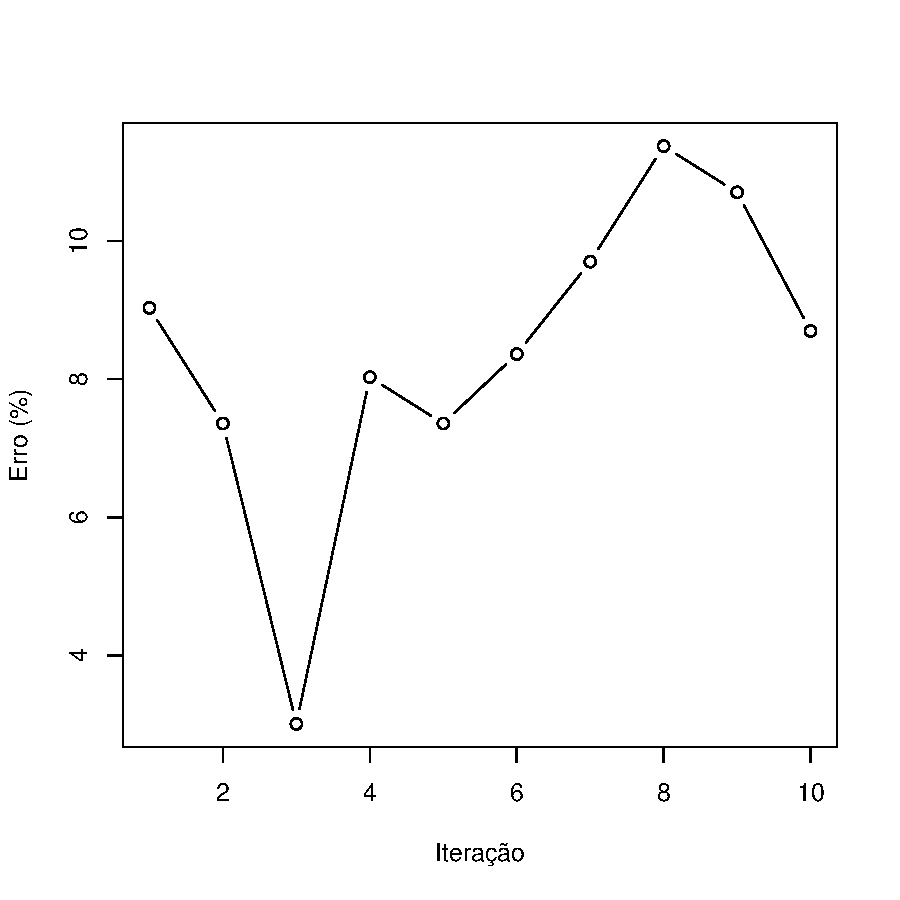
\includegraphics{exercicio6-004}


\end{document}
